\documentclass{bioinfo}
\copyrightyear{2015} \pubyear{2015}

\access{Advance Access Publication Date: Day Month Year}
\appnotes{Manuscript Category}

\usepackage[ruled,vlined]{algorithm2e} % For pseudocode

\begin{document}
\firstpage{1}

\subtitle{Subject Section}

\title[long Title]{Biorseo: Benchmarking ways to use RNA modules leads to improved secondary structure prediction with pseudoknots}
\author[Sample \textit{et~al}.]{Louis Becquey\,$^{\text{\sfb 1,}*}$, Eric Angel\,$^{\text{\sfb 1}}$ and Fariza Tahi\,$^{\text{\sfb 1}}$}
\address{$^{\text{\sf 1}}$IBISC, Univ Evry, Universite Paris-Saclay, 91025, Evry, France}

\corresp{$^\ast$To whom correspondence should be addressed.}

\history{Received on XXXXX; revised on XXXXX; accepted on XXXXX}

\editor{Associate Editor: XXXXXXX}

\abstract{\textbf{Motivation:} RNA loops have now been modelled and clustered from solved 3D structures into ordered collections of recurrent non-canonical interactions called "RNA modules", available in databases. This work explores what information from such modules can be used to improve secondary structure prediction.\\
\textbf{Results:} We propose a Pareto-based method for predicting RNA secondary structures by minimizing a bi-objective both energy-based and knowledge-based potential. The tool, called \textsc{Biorseo}, outputs the secondary structures from the Pareto set. We use it to compare several approaches to predict secondary structures using inserted RNA modules information: two different module data sources, Rna3Dmotifs and The RNA 3D Motif Atlas, and different ways to score the module insertions are compared: module size, module complexity, or module probability according to models like JAR3D and BayesPairing. We benchmark them against 344 known secondary structures. Some of the tested methods present a good performance, especially on structures containing pseudoknots. They are compared to state of the art tools for secondary structure prediction.\\
\textbf{Availability:} The software is freely provided for Linux download on \href{https://evryrna.ibisc.univ-evry.fr/evryrna/biorseo/}{EvryRNA}, with the datasets. \\
\textbf{Contact:} \href{louis.becquey@univ-evry.fr}{louis.becquey@univ-evry.fr}\\
\textbf{Supplementary information:} Appendices A,B and C are available at \textit{Bioinformatics}
online.}

\maketitle

%%%%%%%%%%%%%%%%%%%%%%%%%%%%%%%%%%%%%%%%%%%%%%%%%%%%%%%%%%%%%%%%%%%%%%%%%%%%%%%%%%%%%%%%%%%%%%%%
\section{Introduction}
Ribonucleic acid (RNA) is a macromolecule which is often single-stranded. Therefore, the strand has the ability to fold in space in more complex ways than DNA, that we mostly know to form double-stranded stems. A stem is a succession of basepairs called Watson-Crick basepairs, or "canonical", stacked on top of each other. As this can still happen with RNA, we also observe several other ways for a nucleotide to interact with another. For example, \citealp{leontis2001geometric} proposed a classification of 12 non-canonical basepairs. Some of the nucleotides can also interact with the 2'OH of a ribose, or with a phosphate, or even not interact at all and bulge out the RNA structure.
   
\paragraph{Modelling RNAs as graphs.} ~ 
For modelling purposes, researchers working on computational problems involving RNA represent them with graphs.  A recent article~(\citealp{schlick2018adventures}) details the different graph models of RNAs and their respective advantages. 
We are particularly interested in the secondary structure graph of the RNA, i.e. a graph where the nucleotides are nodes, and backbone bonds and canonical basepairs are edges. In this kind of graph, the non-canonical interactions do not appear. 
As the problem of predicting the 3D structure of an RNA from sequence has been too computationally expensive for years, and is still difficult, a common first step has been to predict this secondary structure (2D) graph, by computing what regions will form stems and what regions will remain unpaired, forming so-called loops. In many cases, the solution to the 2D folding problem is not unique, and RNAs have the ability to switch between several metastable conformations. Most approaches are based on the computation of the RNA partition function and/or canonical pairing probabilities, i.e. the probability for each nucleotide to form a canonical base-pair with every other nucleotide, or to remain unpaired.
In 1990, McCaskill proposed a dynamic programming scheme to compute this partition function~(\citealp{mccaskill1990equilibrium}). The most used implementations are some lower complexity variants of it such as \texttt{RNAFold} in the ViennaRNA package~(\citealp{lorenz_viennarna_2011}), and \texttt{Fold}~(\citealp{mathews2004using}) in the RNAstructure package. An important limitation of this algorithm was its inability to model complex so-called \textit{pseudoknotted} structures, i.e. structures with basepairs $(i,j)$ and $(k,l)$ when $i<k<j<l$. 
Later, some variants taking pseudoknots into account were developped, e.g. in the NUPACK package~(\citealp{dirksAlgorithmComputingNucleic2004}) or \texttt{ProbKnot} from the RNAstructure package~(\citealp{bellaousov2010probknot}).
Once the  partition function is computed, several models exist to rebuild one or several best structure(s): We can choose the Minimum Free Energy (MFE) structure, the one that maximizes expected accuracy (MEA), or the centroid of the ensemble. We can also cite Biokop (\citealp{legendre_bi-objective_2018}), a recent tool that uses both MFE and MEA criterions in a biobjective framework, and returns optimal and suboptimal structures (including pseudoknots).

\paragraph{Secondary structure elements}~ RNAs can be seen as an assembly of stems and loops. To move from the planar 2D graph to 3D, one usually predicts the 3D structure of stems and loops separately. Stems are relatively easy to tackle because of the isostericity of the Watson-Crick basepairs, their structure has been widely observed and features low variability. On the other hand, to accurately model loops in 3D, one needs to take the non-canonical interactions into account. In many cases, two loops can even form new canonical basepairs to form \textit{kissing hairpins}, a particular pseudoknot type (called HHH) which is hard to predict because it involves a distant basepair between two unpaired loop regions.

\paragraph{Modelling RNA loops with more detailed graphs.} ~  Several works have gathered 3D crystal structures involving RNA chains, extracted the loops from those RNA chains and annotated the base contacts using MC-Annotate (\citealp{gendron2001quantitative}), FR3D (\citealp{sarver_fr3d:_2008}) or DSSR (\citealp{lu_dssr:_2015}). They model the loops with more detailed graphs describing non-canonical contacts on their edges. The graphs can then be clustered with respect to a similarity or isomorphism measure, and the sequence variations over the nucleotides of the loop can be modeled. Those models are called RNA \textit{modules}, i.e. an ordered collection of non-canonical basepairs or stacking interactions, leading to a conserved 3D shape in different RNA molecules. We can cite the work from (\citealp{djelloul_automated_2008}) with Rna3Dmotif, a pipeline that extracts terminal hairpin loops, internal loops, and multiple loops from structures annotated by FR3D, and can cluster them using a graph similarity metric. Another one is the RNA 3D Motif Atlas~(\citealp{petrov_automated_2013}), which does not support multiple loops, but clusters the loops using all sequence information, nucleotide contacts and shape information, which leads to loop module models with tolerance in sequence and length variations. A more recent one is CaRNAval (\citealp{reinharz2018mining}), an approach that enables to model a wide variety of structural features such as multipairs, multi-stranded loops, and  pseudoknots. To be exhaustive, we also can cite RNA Bricks 2 (\citealp{chojnowski2014rna}), which has the particularity to also study contacts with protein chains.%, and RNA Motif Scan (\citealp{zhong_rnamotifscan:_2010}) that can search for certain modules in structures, but does not list modules on the form of a database. ==> Is it really relevant ?
These works provide models combining different types of information about a module: (i) a particular base-pairing pattern of canonical and wobble pairing, which is 2D information (it often is only the canonical base-pairs that enclose a loop); (ii) a particular organisation of non-canonical contacts in space, which is 3D information;  (iii) a sequence or consensus sequence that is known to adopt a particular base-pairing organisation, which could be nucleotide probabilities observed in the training dataset of RNA structures, or a more elaborated probabilistic model to predict if a given sequence will fold according to the module.
For example, JAR3D (\citealp{zirbel_identifying_2015}) can score the modules from the RNA 3D Motif Atlas against a query sequence. The recent BayesPairing (\citealp{sarrazin2019automated}), expanding the method proposed by Cruz and Westhof with RMDetect (\citealp{cruz2011sequence}), can be used to do the same on modules from any database by building Bayesian networks from any graph of ordered non-canonical interactions.

\paragraph{Our "backwards" approach} ~ From RNA modules, it is easy to imagine fragment assembly methods which would reconstitute 3D structures from the 2D loops. But this is not our scope here, instead we want to see if that information could be used to predict the position of loops in sequences, in other words, if this knowledge could help predicting the secondary structure graph. Here we finally ignore the 3D information the modules bring. We do not use the 3D data to help sampling conformations, but we use it to score conformations. 

A first attempt to tackle such task, called RNA-MoIP~(\citealp{reinharz_towards_2012}), improves an input secondary structure often given by a simple tool like RNAsubopt~(\citealp{lorenz_viennarna_2011}) to insert modules from Rna3Dmotif into it. The authors have shown that RNA-MoIP produces 2D structures with non-canonical base-pairs included, which are better inputs to give to MC-Sym~(\citealp{parisien2008mc}), resulting in better prediction of 3D structures. Unfortunately, we were not able to reproduce the published results about 2D structure accuracy, probably because the authors used a much older version of RNAsubopt than us. Our own tests over 344 structures with RNAsubopt v2.4.10 + RNA-MoIP showed a slightly inferior performance compared to RNAsubopt alone, as shown in Figure~1\vphantom{\ref{fig:comparison}}. It seems that RNA-MoIP damages the structures predicted by RNAsubopt most of the time, leading to a slightly weaker performance. 
\begin{figure}[!tpb]
\centerline{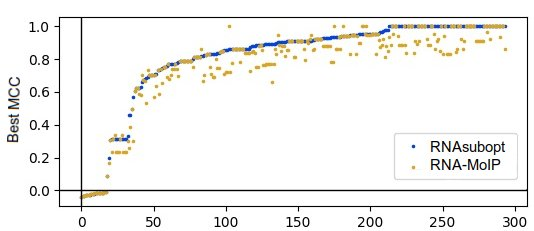
\includegraphics[width=\linewidth]{fig/Figure_1.jpg}} 
\caption{Best Mattews Correlation Coefficient (see equation \ref{eq:MCC}) between the true structure and the structures predicted by RNAsubopt (blue) and RNA-MoIP (yellow) for 344 RNAs of length 10 to 100 from RNA-Strand~(\citealp{andronescu2008rna}). Selection details are provided in section \ref{sec:data}. RNAs are sorted by RNAsubopt performance.}\label{fig:comparison}
\end{figure}
One hypothesis about RNA-MoIP's lack of performance is that it cannot distinguish important base-pairs from less important ones, and might break some of the ones stabilizing a whole stem while inserting a module, resulting in less probable structures as output. 

To test this hypothesis, we design a method which builds a 2D structure by simultaneously placing base-pairs and modules in a single step, taking into account two objectives: the expected accuracy of the structure in the equilibrium ensemble fold, and a custom function that reflects the number and quality of inserted modules (several models are studied). This method leads to our new tool Biorseo (Bi-Objective RNA Structure Efficient Optimizer). Our approach avoids using a weighted linear combination of the objectives as done in RNA-MoIP (which can miss interesting solutions so-called \textit{non-supported} solutions). In this paper, we use a bi-objective Pareto-based approach, i.e. we identify all the non-dominated structures (the structures for which no other structure scores better on the two objectives).

In the next section, this article presents the module models sources, insertion models and objective functions, and the procedure to compare them. Then we present a benchmark of all those variants against reference tools in Section \ref{sec:results}, using a reference dataset (verified structures from the RNA-Strand database). Three well-known reference RNAs are predicted and used to discuss the differences between the methods. %: \textit{E. coli}'s Gln tRNA, the Guanine riboswitch, and the human telomerase's pseudoknot. 
Finally, we recommend two prediction methods, and conclude.

\begin{figure*}[t]
   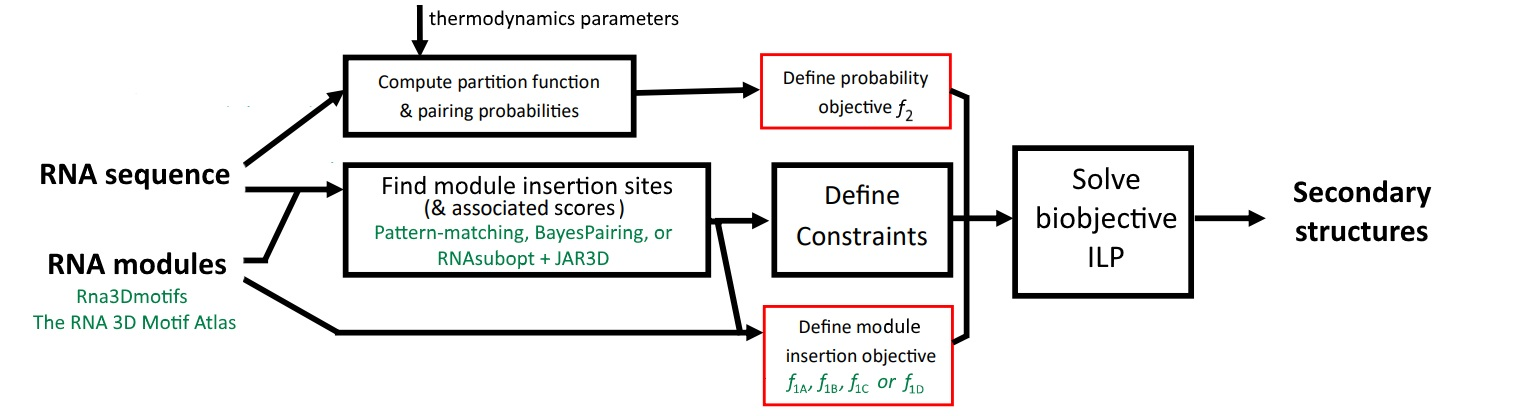
\includegraphics[width=\textwidth]{fig/graph_abstract.jpg} 
   \caption{The information flow in our benchmark method. The inputs are the RNA sequence, and module models from a database. First, we compute the pairing probabilities based on~(\citealp{dirksAlgorithmComputingNucleic2004}) and the probable insertion sites using 3 different methods listed in section \ref{sec:models}. Then, we can define two objectives and linear constraints to compute the Pareto set of secondary structures for that sequence, by solving a bi-objective integer linear program (ILP).}
   \label{fig:pipeline}
\end{figure*}

%%%%%%%%%%%%%%%%%%%%%%%%%%%%%%%%%%%%%%%%%%%%%%%%%%%%%%%%%%%%%%%%%%%%%%%%%%%%%%%%%%%%%%%%%%%%%%%%
\begin{methods}
\section{Methods}\label{sec:methods}
We  compared two databases of modules: (1) Modules extracted from solved 3D RNA structures, in the DESC file format of Rna3dDmotif~(\citealp{djelloul_automated_2008}). We used the data-set provided by RNA-MoIP ~(\citealp{djelloul_automated_2008,reinharz_towards_2012}). (2) Modules from the RNA 3D Motif Atlas v3.2, as provided on the BGSU website ~(\href{http://rna.bgsu.edu/rna3dhub/motifs/}{http://rna.bgsu.edu/rna3dhub/motifs/}), see~(\citealp{petrov_automated_2013}) for more information.

Our main procedure is the following:
\begin{itemize}
\item \textbf{Pattern-matching step:} Find all possible occurrences of known RNA modules in the query sequence, by finding subsequences of the query that score well with the probabilistic models of the modules (several models are compared).
\item \textbf{Constraints definition step:} Define constraints on the secondary structure imposed by modules if they would be included (in this case, some of the canonical base-pairs are forbidden).
 \item \textbf{Optimization step:} Find a secondary structure that satisfies as much as possible both the expected accuracy of the structure and a criterion taking into account module inclusions, by solving a bi-objective integer linear programming problem, using the previous constraints defined in the previous step.
\end{itemize}
  
The linear integer programming framework used to define the constraints and solve the resulting optimization problem is similar to previous works like IPknot, Biokop or RNA-MoIP~(\citealp{sato_ipknot:_2011,legendre_bi-objective_2018,reinharz_towards_2012}), but involves new constraints detailed in appendix A. 
Figure \ref{fig:pipeline} summarizes the procedure on a graphical pipeline.
   
\subsection{Pattern matching step}\label{sec:models}
Several methods have been proposed to tackle the issue of finding if a sequence (or a part of it) is likely to fold following a given module. This section presents the ones we benchmarked.

\paragraph{Direct pattern matching} ~ The simplest approach when no statistical model is available is to use a regular expression and direct pattern matching against the input sequence. This is the approach used by RNA-MoIP. We used it with the Rna3Dmotif data as presented in RNA-MoIP's article ~(\citealp{reinharz_towards_2012}), dealing with special cases in the same way (very short components, wildcards).

\paragraph{The SCFG/MRF method, JAR3D} ~ For each motif group in each release of the RNA 3D Motif Atlas, the BGSU RNA research group proposed to construct a probabilistic model for sequence variability, based on a hybrid Stochastic Context-Free Grammar/Markov Random Field (SCFG/MRF) method. Their implementation, a software called JAR3D ~(\citealp{zirbel_identifying_2015}), takes user-provided loop sub-sequences in input and outputs a score for every motif of the Atlas on every provided loop. This method has the advantage to allow variations in sequence length compared to the module model. Unfortunately, it can only be used for hairpin and internal loops. Another major drawback is that it requires the computation of the pairing probabilities to first locate \textit{where} the most probable loops are, to give them as input to JAR3D. We therefore use RNAsubopt first to get the positions of the probable loops. JAR3D has been developed for modules from the RNA 3D Motif Atlas and can only be tested with them.

\paragraph{Sequence probability distribution and Bayesian Networks} ~ When we have data for several instances of a module, we can estimate a probabilistic distribution of the nucleotides over the module nodes. A first intuitive approach is to use the base frequencies. But as paired nucleotides are not independent at all, it is more rigorous to model those dependencies. An approach proposed in ~(\citealp{cruz2011sequence}) is to transform the module's graph into a Bayesian network, which models the dependencies between nucleotide probabilities at every node of the graph. The original article proposed four hand-made Bayesian networks for only four well-known RNA modules, but a recent tool called BayesPairing ~(\citealp{sarrazin2019automated}) automates the process for every module. A large number of sequences are sampled using the Bayesian network, and they are pattern-matched against the query to find occurrences. An additional step compares the free energy of the structure with and without the constraint of each matched module, and selects only the candidate sites that do not deteriorate too much the energy. This last step is embarrassing for us, first because it requires two computations of the partition function, and then because we would try to insert modules that were pre-selected to be appropriate. Therefore we chose to ignore this last step and let our optimizer select the pertinent modules in the candidates. BayesPairing can be used for both data sources.


%%%%%%%%%%%%%%%%%%%%%%%%%%%%%%%%%%%%%%%%%%%%%%%%%%%%%%%%%%%%%%%%%%%%%%%%%%%%%%%%%%%%%%%%%%%%%%%%%%%%
\subsection{Constraints definition step and IP model} \label{sec:ip}
The full list of variables we used to model the problem in an integer linear program and the linear formulation of each constraint are detailed in Appendix A. Here we propose different objective functions to maximize, whose performances are compared in section \ref{sec:results}.

\paragraph{Notations} ~ We call a \textit{component} a piece of strand which forms an unpaired portion of a module. Components of a module are linked together by canonical base-pairs at their extremities to form a loop. Let $x$ be a module which could be inserted at some defined position in the sequence. Let $\|x\|$ bet the number of components of this module, and $k_{x,i}$ the nucleotide count of the $i$th component of $x$. When a scoring model is used (JAR3D or BayesPairing), we denote $p(x)$ the score value of $x$ inserted at the defined position. Let $p_{uv}$ be the probability for nucleotides $u$ and $v$ (with $v>u+3$) to form a canonical base-pair. We use NUPACK's dynamic programming scheme~(\citealp{dirksAlgorithmComputingNucleic2004}), which supports pseudoknots, to compute such probabilities. We denote $y^u_v$ the binary decision variable indicating that these nucleotides do form a canonical base pair, and $C^x_1$ the decision binary variable indicating whether the module $x$ will be inserted or not. The resolution of the linear program outputs solutions by fixing definitive values for the different $y^u_v$ and $C^x_1$. 

\paragraph{Objective functions} ~ The more modules that are included, the more information about set and unset base-pairs, and the more information we have about the tertiary folds of these loops in space. So maximizing the number of modules could be a valid criteria. But, a disadvantage of such a criteria is that it penalizes multiple loops - sometimes referred as $k$-way junctions - with large $k$, because the insertion of a multiple loop forbids at the same time the insertion of several internal loops or bulges ($2$-way junctions) in place. RNA-MoIP uses the sum of the squared nucleotide count over the components to try to encourage large modules~(\citealp{reinharz_towards_2012}). This is our first benchmarked criteria $f_{1A}$, see equation \ref{eq:A}. Conversely, we could also try to maximize the number of components $\|x\|$ in the module. Then, we can suppose that secondary structure contacts are local (forget about kissing hairpins here), and want to avoid very-long-range base-pairs. This is equivalent to say that we want the minimal loop size (conversely to RNA-MoIP). Therefore, we can penalize a module insertion by the logarithm of the number of nucleotides involved in the looped zone (sum of the $k_{x,i}$) to avoid very long unpaired zones. We introduce such a penalty in criteria $f_{1B}$.\\ We also define two more criteria, $f_{1C}$ which use only the score returned by JAR3D or BayesPairing, and $f_{1D}$ which includes all the presented terms.\\
Let $X$ be the set of all our decision variables, then the different objective functions to maximize are:
\begin{equation} f_{1A}(X) = \sum_{x} \sum_{i=1}^{\|x\|} k_{x,i}^2 \times C^x_1\label{eq:A}\end{equation}
\begin{equation}f_{1B}(X) = \sum_{x} \left[ \frac{\|x\|}{\log_2(\sum_{i=1}^{\|x\|}k_{x,i})} \times C^x_1 \right] \label{eq:B}\end{equation}
\begin{equation} f_{1C}(X) = \sum_{x} p(x) \times C^x_1 \label{eq:C}\end{equation}
\begin{equation}f_{1D}(X) = \sum_{x} \left[ \frac{\|x\|}{\log_2(\sum_{i=1}^{\|x\|}k_{x,i})} \times p(x) \times C^x_1 \right]\label{eq:D}\end{equation}

Regarding the second objective, aimed at maximizing the expected accuracy of the structures, we use $f_2(X) = \sum y^u_v \times p_{uv} \times I[p_{uv}>\theta]$. As first proposed by~(\citealp{sato_ipknot:_2011}), $f_2$ uses a parameter $\theta = 0.001$ to ignore very unlikely base-pairs. This prevents the explosion of the number of variables and allows a fast resolution of the IP problem.

%%%%%%%%%%%%%%%%%%%%%%%%%%%%%%%%%%%%%%%%%%%%%%%%%%%%%%%%%%%%%%%%%%%%%%%%%%%%%%%%%%%%%%%%%%%%%%%%%%%%

\subsection{Optimization step}
We use a simple dichotomic search algorithm (presented in Figure \ref{fig:findP}) to find the Pareto set of the bi-objective problem. On the first pass of the dichotomy, it solves iteratively a mono-objective problem with a constraint on the second objective, requiring it to be in an interval $[\lambda_{min}, \lambda_{max}]$. For example, if we decide to maximize objective 1, every-time a new non-dominated solution is found, $\lambda_{min}$ is set just above the new solution's objective 2 value, to search another one with a worse objective 1 value but a higher objective 2 value than previously found solutions. The second pass of the dichotomy searches below newly found solutions. In fact, it is required to search for superposed solutions to Pareto optimal ones. This is important when the criteria used to rank inserted modules is not able to separate them very well; many solutions therefore get the same $f_1$ score.

The algorithm is implemented  in C++ using the CPLEX solver concert technology~(\citealp{cplex}), resulting in the Biorseo tool, which is available online for Linux platforms.
\begin{figure}[!tbp]
\begin{algorithm}[H]
F:= $\emptyset$\;
\tcp{find the extrema of the Pareto front:}
L1:= maximize($f_1$, $-\infty$, $+\infty$, F)\;
L2:= maximize($f_2$, $-\infty$, $+\infty$, F)\;
\tcp{Add L1 to the results:}
R:= $\{$L1$\}$\;
\tcp{search on top of L1:}
search\_between($f_2(\text{L1}) + \epsilon$, $f_2(\text{L2})$)\;
\tcp{search if solutions superposed to L1 exist:}
search\_between($-\infty$, $f_2(\text{L1})$)\;
\Return{R}\;
\caption{FindParetoSet()}
\end{algorithm}

\begin{algorithm}[H]
$s$:= maximize($f_1$, $\lambda_{min}$, $\lambda_{max}$, F)\;
\If{$s \neq \emptyset$}{
   F:= F $\cup \{s\}$\;
   \If{$\nexists x \in \mathrm{R}$ such as $x>s$}{
         \tcp{solution is undominated, add it to R}
       R:= R $\cup \{s\}$\;
       \While{$\exists x \in \mathrm{R}$ such as $s>x$}{
             \tcp{remove dominated solutions}
           R:= R$\setminus \{x\}$\; 
       }
         \tcp{search on top of $s$}
       search\_between($f_2(s) + \epsilon$, $\lambda_{max}$)\;
       \If{$\lambda_{max} - \lambda_{min} > \epsilon$}{
             \tcp{search if another solution superposed to $s$ exists}
           search\_between($\lambda_{min}$, $f_2(s)$)\;
       }
   }
}
\caption{search\_between($\lambda_{min}$, $\lambda_{max}$)}
\end{algorithm}

\caption{The dichotomic search algorithm to find the Pareto set. F is the ensemble of already-found structures which grows over time, and that we forbid the solver to find again. R is the set of Pareto-optimal solutions. L1 and L2 are the best solutions to the mono-objective problems regarding $f1$ and $f2$. $\mathbf{maximize}$($f$, $\lambda_{min}$, $\lambda_{max}$, F) is a procedure that minimizes the function $f$ (mono-objective IP problem) under the constraint that the other one has to be in interval $[\lambda_{min}$, $\lambda_{max}]$, and with the solutions in F forbidden. The inequality sign $a>b$ between two solutions denotes that solution $a$ dominates solution $b$.}\label{fig:findP}
\end{figure}

\end{methods}

%%%%%%%%%%%%%%%%%%%%%%%%%%%%%%%%%%%%%%%%%%%%%%%%%%%%%%%%%%%%%%%%%%%%%%%%%%%%%%%%%%%%%%%%%%%%%%%%%%%%
%%%%%%%%%%%%%%%%%%%%%%%%%%%%%%%%%%%%%%%%%%%%%%%%%%%%%%%%%%%%%%%%%%%%%%%%%%%%%%%%%%%%%%%%%%%%%%%%%%%%
\section{Results}\label{sec:results}
\begin{figure*}[!tbp]
   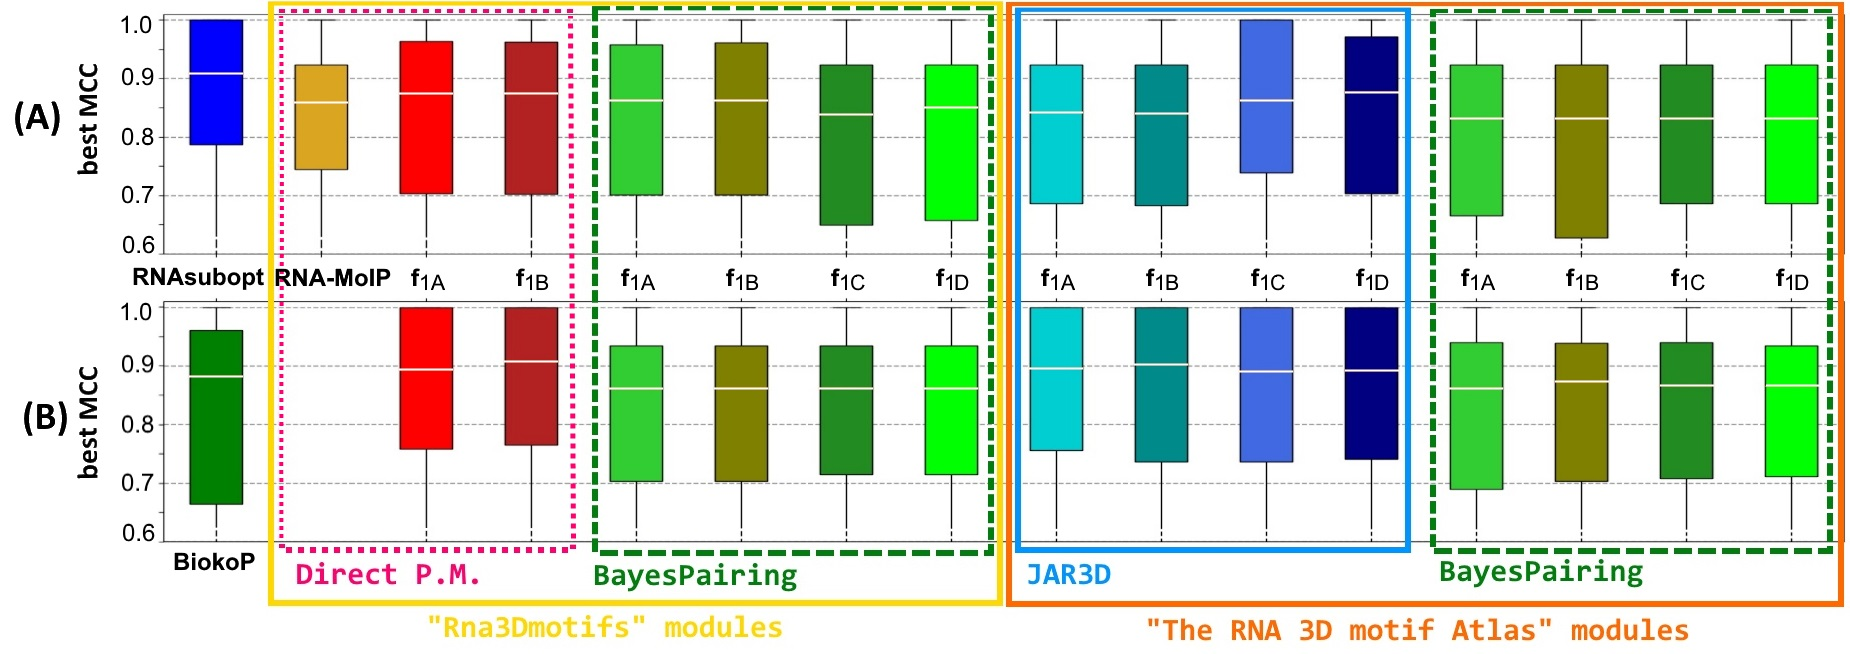
\includegraphics[width=\textwidth]{fig/Benchmark.jpg}
   \caption{Boxplots of the best MCC over the proposed solutions for each of the RNAs, for all method variants. Line (A) shows the methods that cannot find pseudoknots: RNAsubopt, RNA-MoIP, and the 14 variants of Biorseo's bi-objective methods with a constraint that explicitly forbids pseudoknots. Line (B) shows methods which allow their prediction: Biokop, and the 14 variants without the no-pseudoknot constraint. The left block gathers methods which use module data from Rna3Dmotifs (\citealp{djelloul_automated_2008}). The right one gathers those which use modules from the RNA 3D Motif Atlas (\citealp{petrov_automated_2013}). Boxplots surrounded by a dotted red frame use direct pattern matching to detect insertion sites, but do not score the sites. Those surrounded by a continuous blue frame score the sites with JAR3D (\citealp{zirbel_identifying_2015}) to score modules on loop sequences found by RNAsubopt. The remaining surrounded by a dashed green frame use the BayesPairing score~(\citealp{sarrazin2019automated}).}
   \label{fig:upgrades}
\end{figure*}
All the methods introduced return an ensemble of possible secondary structures for a given input sequence. We compare them in a benchmark over short RNA structures and a few well-known application cases. 
\subsection{Benchmark protocol} \label{sec:bench}

\paragraph{Materials}
The tool can be used by a regular scientist on a desktop computer. All computations were performed on a workstation (16 threads @4.3GHz) CPU, 16 GB of RAM. The RAM typically limits the size of the RNAs the methods can process. RNAs up to 230 bases are fine in our case. A prediction typically takes a few seconds, sometimes minutes. The time required grows with both the nucleotide count and the number of loops. The objective functions $f_{1A}$ and $f_{1B}$ were sometimes not discriminative enough and equally ranked a large number of module propositions, leading to combinatorial issues. For that reason, we arbitrarily stopped the jobs exceeding 500 structures in the Pareto set, because they would require over 2 hours of computation time to complete. 

\paragraph{Data sources} \label{sec:data}
A first dataset of RNA secondary structures was extracted from the RNA-Strand database ~(\citealp{andronescu2008rna}). We selected the RNAs for which experimental proof of the structure exists, with size varying between 10 and 100 nucleotides. Sequences containing modified nucleotides (P, T, I in our case) were discarded. The resulting set contains 334 secondary structures of various RNA families, 74 of them containing pseudoknots. We repeated the experiments twice: first, by forbidding explicitly the formation of pseudoknots with additional constraints (for fair comparison with RNA-MoIP). Then, a second one without such limitation, to reach maximum performance. Due to the combinatorial issues described above, only 291 (resp. 294) of the RNAs have been predicted by all the proposed methods (the missing ones often being a combination of direct pattern-matching or JAR3D with $f_{1A}$ or $f_{1B}$) when forbidding (resp. allowing) pseudoknots. We will use these set of results for comparison. \\
In addition, we add a second collection of 264 pseudoknotted-only RNAs from the Pseudobase database~(\citealp{van2000pseudobase}), covering all pseudoknot families, of length also comprised between 10 and 100 nucleotides.\\
To complete the large benchmark, we have a deeper look at very-well known structures to check if relevant combinations of models are still able to predict them correctly.
We used a Gln tRNA from E. coli (RNA-Strand code PDB\_00376), a Guanine riboswitch (RNA-Strand code PDB\_01023), and the pseudoknot of the human telomerase (PDB\_00857). The tRNA is unpseudoknotted, the G riboswitch contains a hard-to-predict HHH type pseudoknot, and the telomerase pseudoknot is a simple H type pseudoknot.

\paragraph{Reference comparison methods}
To study the usefulness of the data sources, objective functions, and module placement methods, we added state-of-the art tools to the comparison. The same RNA sequences were submitted to RNA-MoIP for direct performance comparison. We used RNAsubopt as a reference method without pseudoknot support, because it is fast, widely used, easy to understand and returns several solutions. We used Biokop, the bi-objective integer programming framework, as a reference method for prediction of secondary structures with pseudoknots. Both tools over-perform other state-of-the-art tools in their respective categories, see the appropriate papers (\citealp{lorenz2011viennarna, legendre_bi-objective_2018}) for more benchmarks against other tools.

\paragraph{Metrics} ~ We compute the Matthews correlation coefficient (MCC) between the real secondary structure and every proposed structure. The coefficient is defined as
\begin{equation}
   MCC = \frac{TP. TN - FP. FN}{\sqrt{(TP+FP)(TP+FN)(TN+FP)(TN+FN)}}. \label{eq:MCC}
\end{equation}
Then, we keep the best MCC value found over the set of proposed structures as a metric of the method's performance. This reflects if the true structure is included or not in the Pareto set. Here, we measure if one of the states, which is reported in RNA-Strand as "true" structure, has been found. For comprehensiveness, results with average MCC are also provided in Appendix B, but it is hard to interpret what this average MCC represents. The choice of MCC over accuracy or F1 score is justified by the very large difference between the size of the classes: there exist much more negative base-pairs (pairs of nucleotides that do not interact) than positive ones in any secondary structure.

\subsection{Benchmark results}
Performance results under the form of best MCC are summarized in Figure \ref{fig:upgrades}.
Majority of the RNAs were predicted with similar performance among the methods, including methods that do not use module information. 

No data source, nor objective function taken alone performs significantly better than the other ones. 

\paragraph{Methods without pseudoknots, comparison to RNAsubopt} ~ No method reaches RNAsubopt's scores. The most performing model is the use of the RNA 3D Motif Atlas modules, placed with JAR3D, and scored only with the JAR3D score ($f_{1C}$). We also notice that the 4 models (including this one) which use JAR3D return very small sets of results, most of them being one optimal solution, while RNAsubopt returns from one to ten solutions (with our dataset and default settings).

\paragraph{With pseudoknots, comparison to Biokop} ~ The number of solutions returned doubles for every method compared to its no-pseudoknot version. Most of the RNAs are predicted with small knots as the method allows it. As the bottom line of Figure \ref{fig:upgrades} shows, the methods which use BayesPairing do not find as many right structures than  Biokop, which performs better even without module information. On the other hand, the methods which use direct pattern-matching (like RNA-MoIP did) and the four ones which use RNAsubopt+JAR3D reach higher performance. The largest improvements concern Biorseo + Rna3Dmotifs + $f_{1B}$ and Biorseo + The RNA 3D Motif Atlas + JAR3D + $f_{1B}$. We apply Wilcoxon signed rank tests (non-parametric test for paired samples) to assert these methods distributions of results differ from Biokop (null hypothesis: "The position parameter of the distribution of the differences between the two paired samples is null"): p-values are $1.5\times 10^{-2}$ for the first method using Rna3Dmotifs, and $2.5\times 10^{-3}$ for the second with JAR3D. Other methods have smaller improvements in average, so we do not provide all the statistical tests results.

\begin{figure}[t]
\centerline{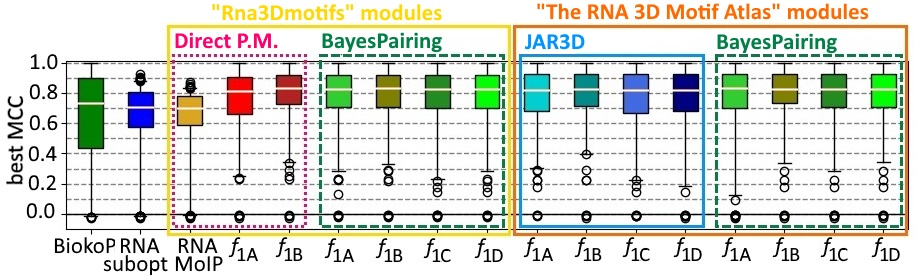
\includegraphics[width=\linewidth]{fig/pseudobase_zoom.jpg}} 
\caption{Boxplots of the best MCC found by the different predictors, on the dataset of 264 pseudoknotted-only RNAs from Pseudobase~(\citealp{van2000pseudobase}. Some computations are incomplete; Biokop succeeded for 201 RNAs, JAR3D+$f_{1A}$ for 249, and JAR3D+$f_{1B}$ for 248. \label{fig:pseudobase}}
\end{figure}
The results on the dataset of pseudoknotted-only structures are presented on Figure~\ref{fig:pseudobase}. Whatever the Biorseo variant, the median best MCC is over 0.8, which is a significant improvement compared to Biokop (0.73, with larger variance). However, the variants are very similar and again, no module source, pattern-matching method nor objective function distinguishes itself.

\subsection{Results of the study cases}
The results about very well described structures are consistent with the general benchmark. Biorseo used with Rna3Dmotifs and direct pattern matching predicts 2D structures as well as RNAsubopt. So does it when used with the RNA 3D Motif Atlas and JAR3D. BayesPairing has a low performance when used with Rna3Dmotifs and a surprising good performance with the Motif Atlas, which cannot be generalized given the larger benchmark data.
The tRNA is an example of structure which is approximately correctly predicted by Biorseo, as well as other tools. The G riboswitch allows to show that Biorseo is less likely to insert false positive pseudo-knots than Biokop (which inserted several, resulting in a low score). 
The telomerase pseudoknot is correctly predicted by all methods that support pseudoknots, including Biorseo. 
Detailed results including structures, number of solutions and computation times are provided in appendix C. 

%%%%%%%%%%%%%%%%%%%%%%%%%%%%%%%%%%%%%%%%%%%%%%%%%%%%%%%%%%%%%%%%%%%%%%%%%%%%%%%%%%%%%%%%%%%%%%%%%%%%
%%%%%%%%%%%%%%%%%%%%%%%%%%%%%%%%%%%%%%%%%%%%%%%%%%%%%%%%%%%%%%%%%%%%%%%%%%%%%%%%%%%%%%%%%%%%%%%%%%%%
\section{Discussion}

\paragraph{Without pseudoknots, comparison to RNA-MoIP} ~  An interesting point is the improvement between RNA-MoIP and the bi-objective method which uses direct-pattern matching to spot insertion sites and $f_{1A}$ to score the insertions. This method only differs from RNA-MoIP because it is bi-objective. The improvement is small, but statistically significant with a Wilcoxon's signed rank test p-value of 0.024. Then, we can conclude that the Pareto approach really improves the structure prediction by itself. This result supports our hypothesis about RNA-MoIP breaking important basepairs. Unfortunately, this improvement in average is counterbalanced by an increase in variance.

\paragraph{Regarding pseudoknots} ~ The support of pseudoknots allows an increase in performance, because we return more solutions, some with pseudoknots, and some without. As we are looking at the maximum MCC here, the appropriate solution has been selected for each RNA. 
Biorseo's reduced number of false positive pseudoknots compared to Biokop can be explained directly by the insertion of modules in loops: as we forbid explicitly any base-pair on nucleotides inside an inserted module's component, we prevent known loops to form pseudoknots. The drawback of this selectivity is the low ability to predict kissing hairpins (HHH type pseudoknots), precisely because they require loops to interact, which happened with our G riboswitch prediction. But for general purpose, given the performance difference between Figures \ref{fig:upgrades} and \ref{fig:pseudobase}, it seems that Biorseo is better on pseudoknotted RNAs.
However, pseudoknot prediction quality is difficult to assess with a metric like MCC, because a pseudoknot could be involved in only two or three base-pairs. Finding them or not does not alter much the MCC even if the structure is much more right or wrong from a biological point of view. Unfortunately, no automated verification method exist yet. A more accurate description of pseudoknot prediction performance would have required manual validation of every occurrence in every structure, which is too much work to achieve on such large datasets.

\paragraph{On the objective functions} ~ 
Regarding objective functions to include modules, the different criteria proposed seem to give comparable results at first sight regarding the average performance and the dispersion. However, an important difference between $f_{1A}$, $f_{1B}$ on one side, and $f_{1C}$, $f_{1D}$ on the other side, is about the computation time. As $f_{1A}$, $f_{1B}$ do not use a score to rank potential module insertion sites, every modules of the same size can be equally inserted. When the RNA presents several loops, the combinatorial possibilities grow fast with the number of modules in the dataset. Therefore, the number of undominated solutions can reach several hundreds or thousands even for short sequences. As evocated in section \ref{sec:bench}, some of the computations never ended because of combinatorial issues with those objectives. Such large Pareto sets are not informative for our application, because they consist in very redundant secondary structures with different module references, which are counted only for one secondary structure solution at the end. On the other hand, $f_{1C}$ and $f_{1D}$ require the run of an additional tool (JAR3D or BayesPairing) to score the insertion sites. Given an RNA, a compromise must be found according to its length and amount of loops.

\paragraph{The bias with JAR3D} ~ One should keep in mind that JAR3D takes as input the sequences of RNA loops to score modules against them. We detected the loops in the RNA sequence with RNAsubopt. This use of JAR3D is biased, because we score modules on sequence portions that we already know unlikely to form stems and likely to form loops. Therefore, the information brought by the insertion of a module is low. 
Then, the enthusiasm about the bi-objective method with JAR3D and $f_{1C}$ (without pseudoknots) has to be moderate. It actually outputs almost the same secondary structures than RNAsubopt, discarding certain ones sometimes. As that method was the only interesting result without pseudoknots, we can argue that including known modules is not a general way to improve secondary structure prediction without pseudoknots. For every method, the median best MCC is below RNAsubopt, and the performance gain obtained on some structures is counterbalanced by the loss on approximately the same number of RNAs or more.

We also observe that using The RNA 3D Motif Atlas with JAR3D has a significantly different behavior than the other methods: first, it returns a very small number of solutions (1 or 2 most of the time). Then, the best structure is almost every-time the one that has the higher number of modules, while it is not the case for the other methods. This is a good point for method JAR3D-$f_{1C}$ which performs almost as well as RNAsubopt by returning only one or two structures. An explanation is that JAR3D is selective of a few module insertion sites, sites that were first perfectly predicted to be loops by RNAsubopt (as discussed earlier). This confirms the use of module information is not always relevant and that the energy criteria brings almost all the information. The modules only sometimes allow to reduce the number of solutions.

\paragraph{About BayesPairing} ~ We want to warn the reader about BayesPairing's low performance here in this benchmark. One should keep in mind that we skipped its last step which checks if the insertion of a module would deteriorate too much the energy. We did so because our bi-objective framework was supposed to be able to do it itself. The low performance of BayesPairing here is not an argument against the tool when used in its intended purpose.

\paragraph{Final choice on which method to use}\label{sec:recommend} ~
The results show that objective functions which use a score on the module insertion site (produced by BayesPairing or JAR3D) require much less computational resources to achieve the computation, as they avoid combinatorial explosion of the number of possible insertions of equally ranked modules onto the different loop sites of the RNA.
On the other hand, they require time to score the modules against the insertion sites.
For that reason, we recommend three models : if the user does not expect pseudoknots, using RNAsubopt is recommended. If the sequence may contain some, we recommend the simplest best-performing model : direct pattern matching and function $f_{1B}$. If the computation is too long because of combinatorial issues, one may use JAR3D to further rank the insertion sites (particularly relevant in longer RNA sequences). We then recommend the use of the RNA 3D Motif Atlas, JAR3D, and function $f_{1B}$. The user also should expect much less solutions when using JAR3D.

%%%%%%%%%%%%%%%%%%%%%%%%%%%%%%%%%%%%%%%%%%%%%%%%%%%%%%%%%%%%%%%%%%%%%%%%%%%%%%%%%%%%%%%%%%%%%%%%%%%%
%%%%%%%%%%%%%%%%%%%%%%%%%%%%%%%%%%%%%%%%%%%%%%%%%%%%%%%%%%%%%%%%%%%%%%%%%%%%%%%%%%%%%%%%%%%%%%%%%%%%

\section{Conclusion}
We developed a general bi-objective method to benchmark different sources of RNA module models (the RNA 3D Motif Atlas and Rna3Dmotifs), different methods to place them in sequences (direct pattern matching, BayesPairing, and JAR3D), and different scoring functions. The bi-objective method uses the expected accuracy of the structure, and the previous scoring functions to select relevant secondary structures.
   
The results show that no data source prevails. They also show that the use of module information is irrelevant to predict structures without pseudoknots. 
The real interest would be when looking for potential pseudoknots, where several of our methods improve the prediction performance (and computation times) compared to state-of-the-art tools.

Some of our models over-perform RNA-MoIP, a previous attempt to predict better secondary structures using module information from Rna3Dmotifs and a linear combination of two objectives into a scoring function. Our simplest best-performing new method could be interpreted as an upgraded RNA-MoIP with a real bi-objective framework and a better module insertion objective, which predicts the base pairs and the module insertions in a row, preventing the insertion to break important base-pairs.

All Biorseo variants are available as a web service or for download on the EvryRNA website.  

Improvement perspectives now rely on the hope than newer databases like CaRNAval~(\citealp{reinharz2018mining}), containing more recent and more diverse module information (there is a 10-fold increase in the number of solved RNA crystal structures between the original Rna3Dmotifs dataset from 2008, and 2018), to really bring more information to assist the energy criteria.\\

\bibliographystyle{natbib}
%\bibliographystyle{achemnat}
%\bibliographystyle{plainnat}
%\bibliographystyle{abbrv}
%\bibliographystyle{bioinformatics}
%\bibliographystyle{plain}

\bibliography{references}


\end{document}
